% !Mode:: "TeX:UTF-8"

\chapter{内存管理模块设计与实现}[memory]
\label{chapter:memory}

\section{模块概述}

Moonix采用两种粒度来对可用的内存进行管理。一种是动态内存分配,另一种是按页进行的内存分配。动态内存分配用于在运行时程序主动请求少量内存的情况。对Moonix来说,动态内存分配的目标是BSS段中一个8 MB大的内存空间;对于应用程序来说,应用程序运行环境也为每个进程都提供了一片内存空间用于动态内存分配。Moonix采用Buddy System Allocation算法来对堆空间进行管理,并按照最小64字节的粒度对堆空间进行划分分配。按页内存分配的分配主体是除去内核以外的所有空闲物理内存,Moonix使用一棵线段树来维护这段内存空间的使用情况。这两种分配都采用外挂式数据结构实现,以降低侵入性和代码耦合度。Moonix同样需要借助按页内存分配来实现物理内存映射到虚拟内存空间。

Moonix采用Rv64架构提供的Sv39系统来实现虚拟内存。在操作系统初始化时,Moonix就会将内核映射到虚拟地址空间,并在创建用户进程的时候都会创建独立的虚拟地址空间,即创建不同的页表来表示不同的映射模式。这样可以将不同进程的代码和数据隔离,在切换到进程时,需要切换到对应进程的页表,这部分将在第 \ref{chapter:thread} 章具体描述。

\section{动态内存分配}

\subsection{Buddy System Allocation算法概述}

动态内存分配是在程序运行过程中,程序动态请求内存空间,操作系统响应而进行的内存分配。通常,操作系统会为每个进程分配一块堆内存空间,该进程执行过程中的动态内存分配都在这块内存上进行。那么该使用怎么的策略进行内存分配就成了操作系统亟待解决的问题。

一个很简单的想法就是,我们可以不断地分配最小的可用地址,这样一直分配下去,内存看起来都是连续的。
但是,在此过程中,如果中间有一块内存被回收了,那么这块内存即使是可用的,但是由于其两边都是被占用的内存,这块空闲区间已经无法被扩展,最终形成外部碎片。
随着不断回收和分配内存,整块内存区间可能产生越来越多的外部碎片,以至于某个时刻,我们可能需要分配一块较大的内存,几个外部碎片的空间之和是足够的,但是单个外部碎片是无法满足需要的。这时可能会想到JVM中的标记整理算法,通过将所有可用的内存向一边移动,来减少外部碎片,这种方式的开销较大,因为操作系统不得不同步更改所有代码或数据中的地址。

Buddy System Allocation是一种经典的内存分配算法\cite{DBLP:journals/acta/BrodalDM05},被大量操作系统实现使用,包括Linux。Buddy System将整块内存按2的幂划分成若干小块,并搜索由小块形成的空闲链表并给出所需求的最佳匹配的大小。该算法的优点可以以较小的时间复杂度(O(logN))快速寻找到合适的空闲块,同时可以快速合并两个相邻的同大小空闲块。同时,由于采用最佳适配的策略,使用该算法进行内存分配会产生较少的外部碎片。该算法的缺点是会产生内部碎片,例如如果要分配66个单位,那么必须划分128单位的块,内部多出来的内存空间就无法被使用了。

\subsection{动态内存分配实现}

在Moonix中,内核的动态内存分配主体,是bss段的一块8 MB大小的内存区域。Moonix将最小划分的块定为64字节,这个大小是基于空间上的考虑,将在本节最后给出这种方案的内存开销。

Moonix使用一棵二叉树来存储每一级范围内的最大连续空闲块个数。最底层的节点代表每个最基本的64字节内存块的使用情况,第二层的每一个节点则代表两个64字节内存块,即一个128字节范围的使用情况。以此类推,最顶层的单个节点就表示全部的8 MB大小的内存区域的使用情况。如图 \ref{pic:buddysystem} 所示。

\begin{figure}[htpb]
	\centering
	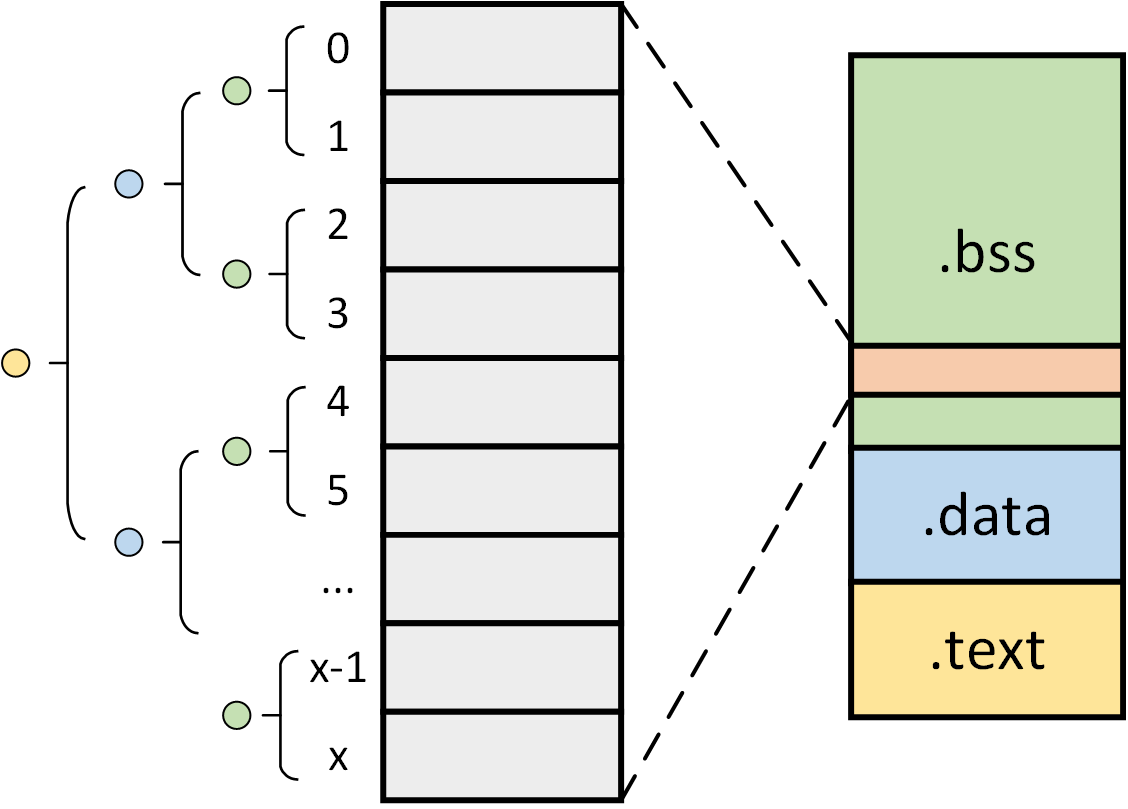
\includegraphics[width=0.65\textwidth]{buddysystem}
	\setlength{\abovecaptionskip}{2pt}
	\caption{保存中断上下文}
	\label{pic:buddysystem}
\end{figure}


\begin{minipage}[c]{0.95\textwidth}
\begin{lstlisting}[language={C}, caption={动态内存分配管理二叉树}, label={lst:mallocbinary}]
struct
{
	int size;
	int longest[BUDDY_NODE_NUM];
} buddyTree;
\end{lstlisting}
\end{minipage}

二叉树的每个节点的值表示该节点所代表的范围内最多可以使用的连续空闲块的个数,这个数值是由该节点下层每一级的节点数值取较大值得出的,原理类似于胜者树的调整过程。Moonix中定义的用于管理动态内存分配的二叉树结构如代码 \ref{lst:mallocbinary} 所示。size域为整棵二叉树管理的总内存块的个数,而longest数值记录了二叉树每个节点的值。其中,BUDDY\_NODE\_NUM的值应当等于$size<<2-1$。\\

\begin{algorithm}[H]
	\SetKwInOut{KIN}{\textbf{输入}}
	\SetKwInOut{KOUT}{\textbf{输出}}
	\KIN{待分配的内存块个数}
	\KOUT{分配的内存区域的首块块号}
	
	设置所需内存块个数为大于等于输入数量的最小的2的幂\;
	设置当前节点为二叉树根节点\;
	\While{当前节点大小 != 所需内存块个数}{
		\eIf{左分支节点较小且满足条件}{
			将左分支节点设置为当前节点\;
		}{
			将右分支节点设置为当前节点\;
		}
	}
	将当前节点的值设为0\;
	将临时节点设置为当前节点\;
	\While{临时节点 != 根节点-1}{
		将当前临时节点的父节点设置为临时节点\;
		将当前临时节点的值设置为左右分支的最大值\;
	}
	返回当前节点对应范围的第一个块号\;
	\caption{动态内存分配}
	\label{alg:kalloc}
\end{algorithm}

\vspace{12 pt}

分配过程对应于算法 \ref{alg:kalloc}。其中算法第四行中优先寻找较小的且满足条件的块,这样分配会尽量保留大块,减小外部碎片。该算法的另一个实现可能会寻找第一个满足条件的块,这样会产生较多的外部碎片而导致分配效率降低。

注意在分配时,只会标记被分配节点的使用情况,而不会修改其下级节点的值,这样是为了在回收时可以快速确定最初被分配出去的节点。

在通过分配算法标记二叉树中的占用情况,并返回第一个块的块号后,即可根据块号和块的大小,计算出相对于堆空间起始地址的偏移,最终得到这块可用内存的地址。

下面来计算使用Buddy System Allocation算法管理堆内存时所需要的额外内存开销。

如果我们想要管理8 MB,即$2^{23} Byte$的内存,最小分配的块大小是$64 Byte = 2^6 Byte$,那么要管理的内存空间可划分为$2^{17}$块,用于管理的满二叉树共有$2^{18} - 1$个节点,每个节点是一个四字节的无符号整数,BuddyTree所占用的内存空间$2^{20} Byte$,即1 MB。Moonix只需要额外花费1 MB内存,就可以管理这8 MB的堆内存空间。

\section{按页内存分配}

按页内存分配的主体是整个可用的物理内存,首先需要确定可用的物理内存范围。Moonix目前运行在QEMU虚拟机模拟的Virt机器上,Virt机器将128MB的物理内存安排在0x80000000到0x88000000空间上。这块可用的内存空间就是按页内存分配的主体。

Moonix使用一棵非递归线段树来对这块内存进行管理。事实上,非递归版本的线段树和第一节提到的Buddy System Allocation算法的结构非常类似,同样也是一棵二叉树管理2的幂级数长度的区间。唯一不同的是,按页内存分配不需要记录该区间上还有多少空闲页,因为一次只分配一页。这样,每个节点只需要记录一个布尔类型的值,即该区间上是否有空闲页。

由于思想基本一致,不再赘述其思想与实现。

\section{虚拟地址空间}

Moonix使用Sv39系统来实现虚拟地址空间,以实现进程间代码数据隔离与共享,并固定进程的内存布局,降低应用程序编写的难度。同时,通过页表还可以提供对特定内存区域的访问控制,以防止恶意应用程序任意读写执行内存。

\begin{minipage}[c]{0.95\textwidth}
\begin{lstlisting}[language={C}, caption={页表相关数据结构定义}, label={lst:pagetable}]
typedef usize PageTableEntry;   /* 页表项长度 64 位 */
/*
* 页表由页表项组成 
* 一页页表中包含 4096 / 8 个页表项
*/
typedef struct
{
	PageTableEntry entries[PAGE_SIZE >> 3];
} PageTable;
\end{lstlisting}
\end{minipage}

Moonix将内核区域分成如表 \ref{tab:sectionprivilege} 所示的几个部分,并分别定义了是否可读可写可执行的访问权限。

\begin{table}[h]
	\centering
	\caption{Moonix中各个段权限}
	\label{tab:sectionprivilege}
	\begin{tabular}{|c|c|c|c|}
		\hline
		段名      & 可读 & 可写 & 可执行 \\ \hline
		.text   & 是  & 否  & 是   \\ \hline
		.rodata & 是  & 否  & 否   \\ \hline
		.data   & 是  & 是  & 否   \\ \hline
		.bss    & 是  & 是  & 否   \\ \hline
		剩余空间    & 是  & 是  & 否   \\ \hline
	\end{tabular}
\end{table}

Moonix中,为了方便操作页表和页表项相关的数据结构,将相关结构定义如代码 \ref{lst:pagetable}。

虚拟内存映射的难点在于,如何递归创建页表结构并填充。Moonix采用一个比较巧妙的方式,在查找页项的同时,如果发现对应层级的页表还没有构造,就动态申请一块内存用作页表,并记录在上层页表项中。这样在映射的过程中,就只会创建使用到的内存区域对应的下级页表,而无需构建全部的页表了。查找页表项并构建所需的下级页表的实现见代码 \ref{lst:createpagetable}。

在完成页表项和页表的构建之后,只需要将根页表的物理页号写入satp寄存器中,CPU就会在取得虚拟地址时,自动地进行地址翻译。

同样,当用户进程执行时,除了要将内核映射到用户进程的高地址处以外,还需要将进程自己的代码和数据映射到虚拟地址空间的低地址位,同时,还需要设置进程的代码和数据的页表项的U标志位,以保证该内存区域可以在U-Mode下访问。

\begin{minipage}[c]{0.95\textwidth}
\begin{lstlisting}[language={C}, caption={查找页表项}, label={lst:createpagetable}]
	PageTableEntry
	*findEntry(Mapping self, usize vpn)
	{
		PageTable *rootTable = (PageTable *)accessVaViaPa(self.rootPpn << 12);
		usize *levels = getVpnLevels(vpn);
		PageTableEntry *entry = &(rootTable->entries[levels[0]]);
		int i;
		for(i = 1; i <= 2; i ++) {
			if(*entry == 0) {
				// 页表不存在,创建新页表
				usize newPpn = allocFrame() >> 12;
				*entry = (newPpn << 10) | VALID;
			}
			usize nextPageAddr = (*entry & PDE_MASK) << 2;
			entry = &(((PageTable *)accessVaViaPa(nextPageAddr))->entries[levels[i]]);
		}
		return entry;
	}
\end{lstlisting}
\end{minipage}

\section{模块测试}

内存管理模块主要测试物理地址映射到虚拟地址空间的过程。编写一测试脚本,以映射main函数的地址为例,测试脚本输出内容如代码 \ref{lst:memtest} 所示。

\begin{minipage}[c]{0.95\textwidth}
\begin{lstlisting}[language={C}, caption={main函数地址翻译}, label={lst:memtest}]
main 函数虚拟地址: 0xffffffff80202d8a
vpn: 0xffffffff80202
level 1: 510
level 2: 1
level 3: 2

satp: 0x8000000000080c30
根页表 ppn: 0x80c30

level 1 条目: 0x000000002030c401
条目表示权限:不可读不可写不可执行
下一级页表ppn:0x80c31

level 2 条目:0x000000002030c801
条目表示权限:不可读不可写不可执行
下一级页表ppn:0x80c32

level 3 条目:0x000000002008080b
条目表示权限:可读不可写可执行
结果ppn:0x80202

加上偏移量得到 main 函数物理地址:0x0000000080202d8a
\end{lstlisting}
\end{minipage}

内核中main函数的虚拟地址为0xffffffff80202d8a,测试脚本模拟CPU查找页表进行地址翻译的过程以验证正确性。CPU的地址翻译以页为单位进行,将虚拟页号翻译为物理页号,main所在的地址的虚拟页号为0xffffffff80202。从虚拟页号中可以分割出该页项在三级页表中的下标,分别是510、1和2。当前CPU的satp寄存器的值为0x8000000000080c30,高位的8表示当前分页采用Sv39系统,低位0x80c30即为根页表的物理页号。

\begin{figure}[htpb]
	\centering
	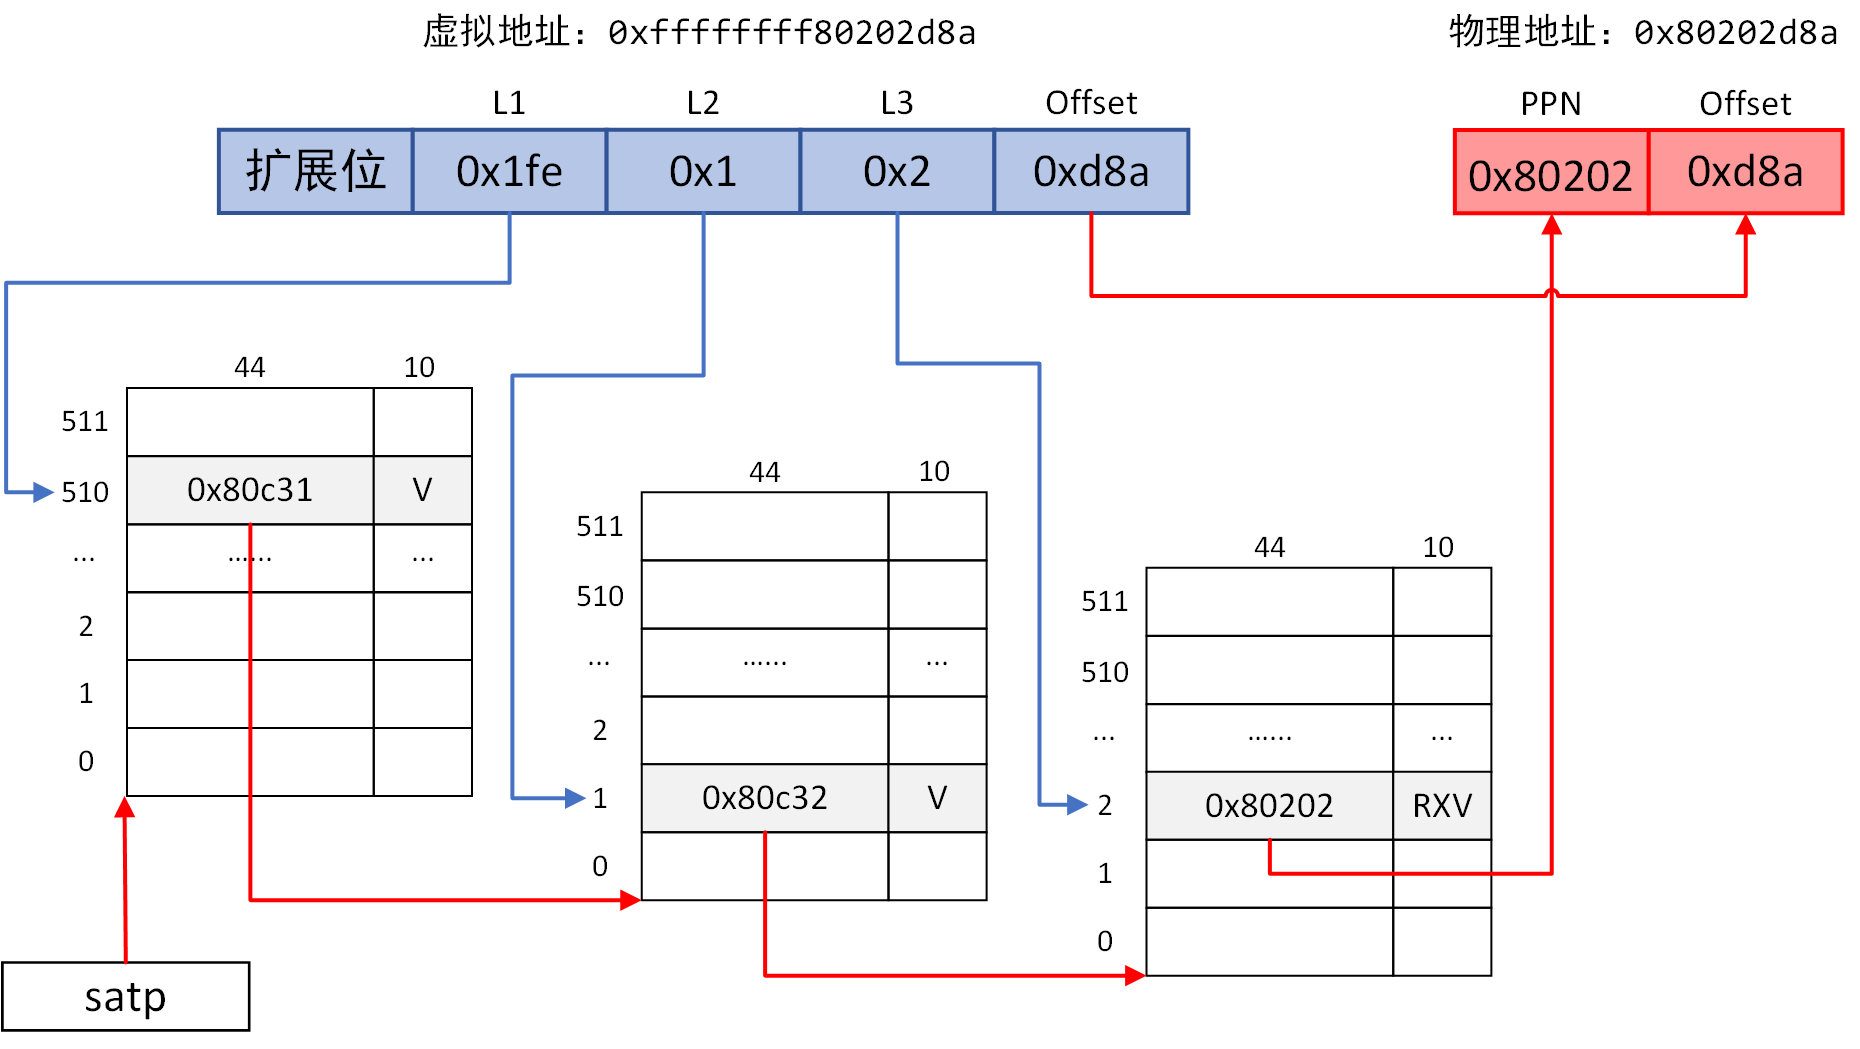
\includegraphics[width=0.9\textwidth]{memtest}
	\setlength{\abovecaptionskip}{2pt}
	\caption{main地址翻译过程}
	\label{pic:memtest}
\end{figure}

有了这些信息,CPU首先从根页表中取出第510条页表项,内容为0x000000002030c401,从中解析出页表项权限为不可读不可写不可执行,表示该页表项指向了下一级页表,下一级页表的物理页号为0x80c31。随后CPU从下一级页表中取出第1条页表项,内容0x000000002030c801,解析后的权限同样是不可读不可写不可执行,指向的下一级页表的物理页号为0x80c32。从第三级页表中取出第2条页表项,内容0x000000002008080b,权限为可读不可写可执行,表示这已经是最终的页表项,解析的结果的物理页号为0x80202,再加上页面内的偏移即可得到main函数的物理地址为0x0000000080202d8a。由于内核是线性映射的,映射偏移恰好是0xffffffff00000000,即可验证整个翻译过程确实是符合预期的。翻译过程如图 \ref{pic:memtest} 所示。